\documentclass[10pt,twocolumn,letterpaper]{article}
%% Welcome to Overleaf!
%% If this is your first time using LaTeX, it might be worth going through this brief presentation:
%% https://www.overleaf.com/latex/learn/free-online-introduction-to-latex-part-1

%% Researchers have been using LaTeX for decades to typeset their papers, producing beautiful, crisp documents in the process. By learning LaTeX, you are effectively following in their footsteps, and learning a highly valuable skill!

%% The \usepackage commands below can be thought of as analogous to importing libraries into Python, for instance. We've pre-formatted this for you, so you can skip right ahead to the title below.

%% Language and font encodings
\usepackage[spanish,english]{babel}
\usepackage[utf8x]{inputenc}
\usepackage[T1]{fontenc}

%% Sets page size and margins
\usepackage[a4paper,top=3cm,bottom=2cm,left=3cm,right=3cm,marginparwidth=1.75cm]{geometry}

%% Useful packages
\usepackage{amsmath}
\usepackage{graphicx}
\usepackage[colorinlistoftodos]{todonotes}
\usepackage[colorlinks=true, allcolors=blue]{hyperref}

%% Title
\title{
		%\vspace{-1in} 	
		\usefont{OT1}{bch}{b}{n}
		\normalfont \normalsize \textsc{Proyecto Final - DYCDE - 2025} \\ [10pt]
		\huge Estación Remota de Química \\
}

\usepackage{authblk}

\author[1]{Leonel Morales De Paz - Carné:23001545}

	\affil[1]{\small{ Ingeniería en Electrónica - FISICC }}

\begin{document}
\maketitle

\selectlanguage{english}

\section{Abstract}
\begin{Abstract}
The creation of printed circuit boards has been a skill that has taken humanity to a much more advanced age, allowing machines that once took up a small space to perform the same functions, but now with a size small enough to fit in the palm of a hand. Chemistry is a very exact science that requires precise data to achieve an expected and favorable result, so it is vitally important to receive accurate information, such as environmental data or even mixtures being made, in order to keep track. Therefore, in this project, we will seek to provide a compact device that allows them to understand their environment and take measurements to obtain ideal results.
\end{abstract} \\ 
\\ 

\section{Resumen}
La creación de placas de circuito impreso ha sido una habilidad que ha llevado a la humanidad a una era mucho más avanzada permitiendo que máquinas que antiguamente ocupaban un espacio puedan ejecutar las mismas funciones pero ahora con el tamaño lo suficientemente reducido como para estar en la palma de una mano. La química es una ciencia muy exacta que necesita de datos precisos para alcanzar un resultado esperado y favorable por lo que es de vital importancia recibir información precisa como bien puede ser datos del ambiente o incluso de mezclas que se esten realizando con el fin de llevar un control por lo que en este proyecto buscaremos proporcionar un dispositivo compacto que les permita conocer su ambiente y tomar mediciones para obtener resultados idóneos.

{\textbf{Keywords} \\
Electronics, IoT, Diseño y Contruscción, Dispositivos Electrónicos}

\section{Descripción del problema}
En diversas industrias un ambiente controlado es algo muy importante para mantener la calidad del producto y en muchos casos para reducir el riesgo laboral. Una de la ciencias más exacta y donde más se podría decir que importa un control preciso de las condiciones es en el área de la química ya que cualquier variación podría generar un producto no deseado, más aún con los procesos más exquisitos y sensibles por lo que buscaremos generar un apoyo a la industría química proporcionando a los usuarios la información sobre el ambiente que los rodea para mantener un mejor control sobre sus condiciones y además generaremos información útil sobre los mismos compuestos tanto como para la correcta elaboración del producto como para la protección del usuario. 

\section{Objetivo General}
Proporcionar la información necesaria para tener las condiciones de laboratorio lo más controladas posibles manteniendo un ambiente seguro y efectivo para la elaboración de diversos compuestos.

\section{Objetivos Específicos}
    - Proporcionar información precisa sobre la temperatura, humedad y presión atmosférica por tanto la altura del lugar en el que se trabajará. 

    - Proporcionar información sobre la temperatura de los compuestos que se están utilizando, para evitar errores o facilitar la obtención de diversos productos.

    - Proporcionar información sobre los gases de escape que puedan generar las reaccines centrandonós en los más comunes propano, metano y alcohol para ser extraidos.


\section{Materiales}
-ESP32
-Sensor BME680 (temperatura, húmedad y presión)
-Relays 3.3V a 120V.
-Sensor DS18B20 medición de temperatura de compuestos.
-Sensor MQ-2.
-Buzzer.
-Neopixeles.

\section{Discusión}
Algo básico sería la medición de temperatura, humedad y presión del ambiente para lo que se utilizará un sensor BME680 para obtener los datos necesarios, en el caso de alcanzar cierta temperatura se activará un relé que activaría un ventilador, los datos de humedad del aire también se registrarán y serán importantes en el control del laboratorio y los datos de la presión serán útiles para determinar la altura a la que se encuentra la estación de química. Para la temperatura de un recipiente se podra utilizar un sensor DS18B20 para detectar la temperatura de la cristaleria donde se realizarán las mezclas de compuestos. Y finalmente para la detección de gases como el humo, metano, propano, alcohol, etc. se utilizará un sensor MQ-2 que nos permitirá encender otro ventilador que extraera dichos gases de la habitación, además, la concentración de gas se determinaría  por el sensor MQ-2 activando un buzzer alertando de la alta concentración de gas en el aire.

\section{Resultados}

A lo largo de este proyecto tuvimos varios inconvenientes como lo fue el tiempo de espera por las placas debido a errores menores que tuvieron repercusiones, además, el ser la primera vez que se implementaba la tecnología smd a este nivel junto a la truhold junto a la implementación de la comunicación MQTT es algo que termino afectando en el desarrollo del proyecto inevitablemente, sin embargo, se lograron cumplir todos los objetivos luego de varias horas de esfuerzo como lo son las mediciones de temperatura tanto para líquidos por medio del DS18B20 como las mediciones ambientales junto a la altura por medio de BME680, se pueden apreciar los valores gráficamente y los neopixeles representan bien las condiciones de dichos componentes activnadose a ciertas temperaturas con colores que identifican si está frío, templado o caluroso, el relé que controlaría un ventilador por medio de los valores de temperatura también funcionó satisfactoriamente, el sensor de gas MQ-2 nos dió más problemas pero se logró hacer funcionar satisfactoriamente, tanto los neopixeles cambiando de verde (seguro) como a rojo (peligroso) si se detecta una concentración de gas peligrosa en el aire como la activación del relé igualmente al alcanzar esas peligrosas concentraciones de gas, la publicación del valor analógicos de gases representando las ppm del gas también tuvo vomplicaciones pero se lograron presentar dichos datos satisfactoriamente, el ESP32 y la comunicación I2C fue todo un éxito alcanzando precisión en las mediciones correspondientes como se tenía esperado, al fin y al cabo luego de mucho esfuerzo se lograron alcanzar todos los objetivos, funcionando la tarjeta perfectamente bien y lista para poder usarse.

También se logró implementar un "batch" por medio de impresión 3D para la placa, manteniendo la estética y generando una portección para la propia placa.


\begin{figure}
  \centering
  \includegraphics[width=0.4\textwidth]{PlacaDycde.jpg}
  \caption{Placa de circuito impreso "Módulo de Química".}
\end{figure}

\begin{figure}
  \centering
  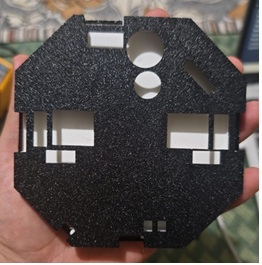
\includegraphics[width=0.4\textwidth]{BatchPlaca.jpg}
  \caption{Batch o cubierta de protección para el "Módulo de Química".}
\end{figure}

\begin{figure}
  \centering
  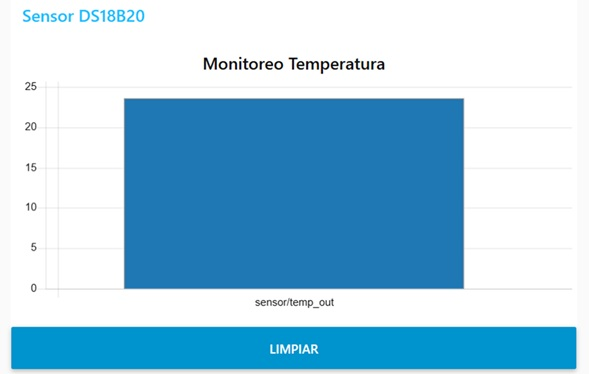
\includegraphics[width=0.4\textwidth]{DS18B20.jpg}
  \caption{Sensor tipo sonda DS18B20 medición de temperatura de compuestos.}
\end{figure}

\begin{figure}
  \centering
  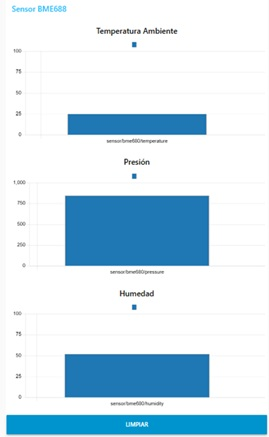
\includegraphics[width=0.4\textwidth]{MedidasAmbientales.jpg}
  \caption{Sensor BME680 medición de temperatura, húmedad y presión.}
\end{figure}

\begin{figure}
  \centering
  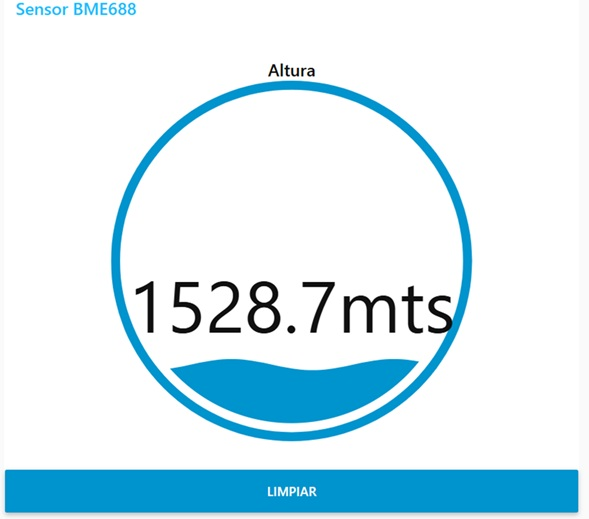
\includegraphics[width=0.4\textwidth]{Altura.jpg}
  \caption{Determinada por la medición de presión del BME680.}
\end{figure}

\begin{figure}
  \centering
  \includegraphics[width=0.4\textwidth]{Gas.jpg}
  \caption{Sensor de gas MQ-2.}
\end{figure}

\section*{Conclusiones}
El sensor DS18B20 es un sensor tipo sonda bastante preciso capaz de otorgarnos mediciones bastantes precisas del líquido o material (siempre compatible con la sonda) a la que se someta, ideal para estar seguro de las temperaturas de las mezclas correspondientes. El BME680 nos permite tener un buen control de nuestro ambiente de trabajo permitiendonos tomar acción en el caso de necesitarlo, además, que por medio de esa información del sensor se activa el relé que puede conectarse a un circuito como el ejemplo principal que era encender un ventilador, además,  tenemos los leds de alerta para temperaturas sobre los niveles esperados y también para niveles de concentración extremas de gases. El sensor MQ-2 tuvo varias complicaciones ya que su funcionamiento era algo confuso como la necesidad de que este se calentará para mediciones más precisas, la falta de numeración en sus terminales y las erraticas mediciones de vez en cuando, pero al final se logró comprender su funcionamiento satisfactoriamente y se implemento sin problemas logrando activar y desactivar el relé y el buzzer. La comunicación del ESP32 funciono perfectamente bien se aprendio de mejor forma a trabajar con componentes smd y se creció en el diseño de circuitos aprendiendo a diseñar batch desde cero con fines específicos, además, se aprendió a lidiar con ciertos inconvenientes o errores que se puedan dar en el proceso de diseño, ensamble y programación.

\section*{Agradecimientos}
A los profesores y compañeros que nos han apoyado mucho en este semestre con el fin de aprender a como ser capaces de crear nuestras propias placas de la mejor forma posible siendo estéticas y funcionales.

\begin{thebibliography}{9}
\bibitem{a_reference} DS18B20 Datasheet(PDF). (s.f.). ALLDATASHEET.COM - Electronic Parts Datasheet Search. https://www.alldatasheet.com/datasheet-pdf/pdf/58557/DALLAS/DS18B20.html

\bibitem{other_ref} Gas sensor BME688. (s.f.). Bosch Sensortec. https://www.bosch-sensortec.com/products/environmental-sensors/gas-sensors/bme688/

\bibitem{other_ref} MQ135 Datasheet(PDF). (s.f.). ALLDATASHEET.COM - Electronic Parts Datasheet Search. https://www.alldatasheet.com/datasheet-pdf/pdf/1307647/WINSEN/MQ135.html

\bibitem{other_ref} (s.f.). OLIMEX LTD - OLinuXino Arduino Maple Pinguino ARM Open Source Hardware Development Boards. https://www.olimex.com/Products/Components/Sensors/Gas/SNS-MQ135/resources/SNS-MQ135.pdf

\bibitem{other_ref} (s.f.). Wireless SoCs, Software, Cloud and AIoT Solutions | Espressif Systems. https://www.espressif.com/sites/default/files/documentation/esp32_datasheet_en.pdf

\bibitem{other_ref} (s.f.). Measuring CO2 Concentration in Air using Arduino and MQ-135 Sensor. (s.f.). Circuit Digest - Electronics Engineering News, Latest Products, Articles and Projects. https://circuitdigest.com/microcontroller-projects/interfacing-mq135-gas-sensor-with-arduino-to-measure-co2-levels-in-ppm




\end{thebibliography}

\end{document}